% !TEX root = report.tex

\chapter{Introduction}

In this report, we are designing and developing a bot that plays the game StarCraft. A StarCraft bot is a computer program or script that plays a game of StarCraft. Our intention for the bot is that it plays without any cheats, adapts to the state of the game and responds quickly. Although we initially pursued the goal of winning as well, we decided to change the focus on being capable of playing properly.

\section{The Game StarCraft}

StarCraft is a real-time strategy game developed by Blizzard and was shipped in 1998. Its foremost expansion Brood War was released later that same year. In general, when one talks about StarCraft, the expansion is implicitly included. Over the years, the game became quite popular as it introduced various interesting gameplay and multiplayer features that easily allowed for communities to grow.

There were three totally different races to be chosen from; the technologic advanced alien race Protoss with access to psionic weaponry and energy shields, the organic alien race Zerg that thrives on evolution and its great numbers to obliterate enemies, and the humanoid race Terran that focuses on conventional weaponry such as machine guns, tanks and nuclear weapons. Each of these races have their own unique units, structures, and how they are to be played. In order to build and train those units, the resources Minerals and Vespene Gas have to be harvested and brought back to the main structure of the player.

The other foremost reason is that it was relatively easy to play online against others. This resulted in communities growing and many contests held, were money was at stake. Eventually, professional StarCraft player became a carreer for some. And in South Korea, the idea of showing games live on television was pioneered, players became celebrities, schools and training houses for teams were organized, and even an official club regulated it as a \emph{sportsmanship}. With the fairly recent introduction of StarCraft II, however, the original game has decreased in popularity. Despite this, the game is still seen as one of the best games of all times.

The game also featured an artificial intelligence, allowing players to try a \emph{skirmish} against the computer. The AI could play at four different levels, ranging from easy to insane. But the AI itself was a very easily programmed script. It did not adapt to the players decisions, was quite repetitive and was easily misled. Furthermore, it cheated by having full observability over the whole field, while the game itself features a \emph{Fog of War} (areas out of sight range are blacked out). It also cheated by having additional resources, allowing it to train units even when economically impaired.

%\begin{figure}
%\centering
%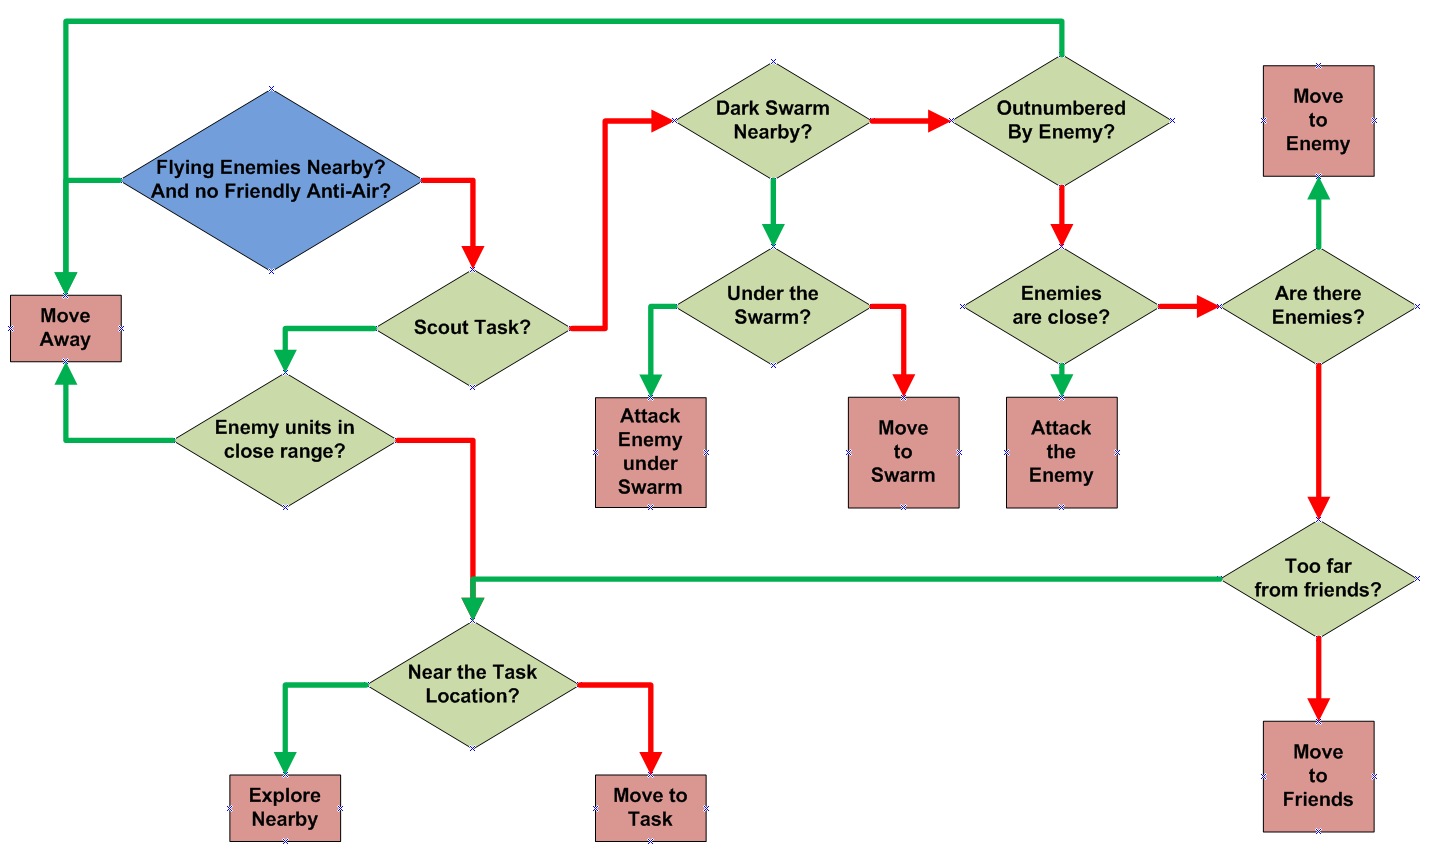
\includegraphics[scale=0.35]{starcraft_zerg_diagram_groot}
%\caption{\label{fig:micro} Flow chart illustration of the decision tree for 'Zergling' units. The blue rhombus is the start and is a decision node. Green rhombi are also decision nodes. Red squares are decision terminals that are to be executed. Green lines indicate a 'yes' answer to the respective question, and red lines indicate 'no'.}
%\end{figure}

\begin{figure}
        \begin{subfigure}[b]{0.5\textwidth}
                \centering
                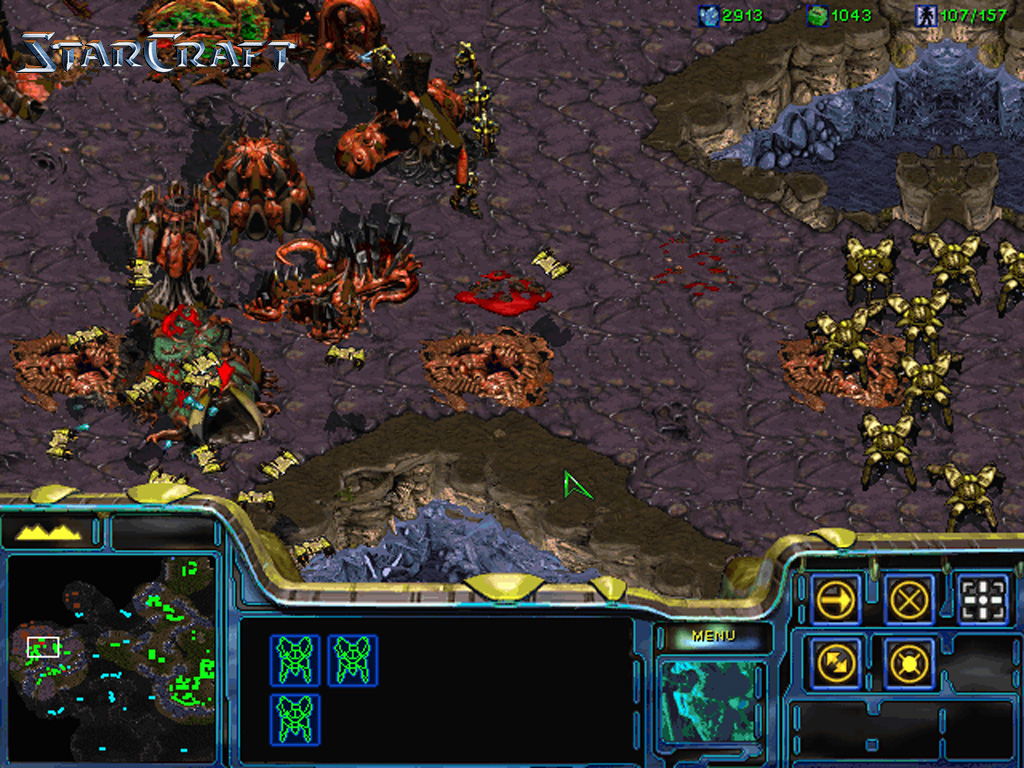
\includegraphics[width=\textwidth]{sc1}
        \end{subfigure}%
        ~ %add desired spacing between images, e. g. ~, \quad, \qquad etc. 
          %(or a blank line to force the subfigure onto a new line)
        \begin{subfigure}[b]{0.5\textwidth}
                \centering
                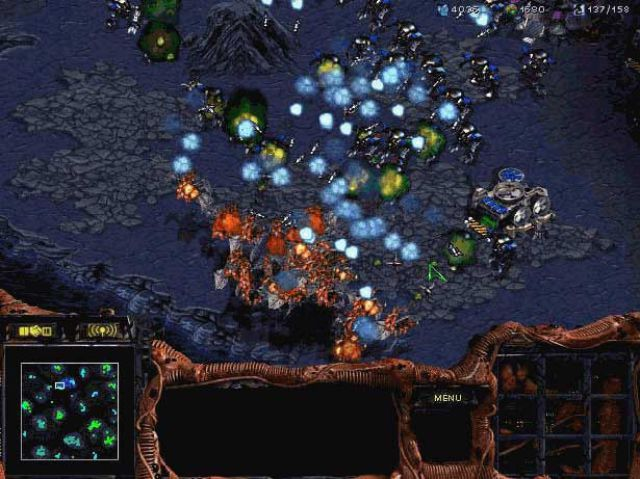
\includegraphics[width=\textwidth]{sc2}
        \end{subfigure}
        ~ %add desired spacing between images, e. g. ~, \quad, \qquad etc. 
          %(or a blank line to force the subfigure onto a new line)
        \caption{Images of battles in StarCraft Brood War}\label{fig:animals}
\end{figure}


\section{Goal of the Bot}
Our goal for the bot is to develop an AI that does not cheat and actually plays the game as it should. To make it more interesting than the standard AI already present in the game, we wanted something that could actually adapt to the game and also made its own strategies.

We arrived at this idea for a project when we stumbled upon an AI competition for StarCraft, AIIDE2010, meant for bots to play each other. There were four different tournaments one could participate in, from very small scale battle to the complete game. The first two focused on team versus team battles. The third one is a simplified game of StarCraft, where both bots play Protoss, have only access to the units of the lowest tier of technology, and have to gather resources to produce units. The focus of this game is on a more strategic level, as units can not run quickly to the other side of the map. As for the fourth, we have a normal complete game of StarCraft. Although people were free to pick any race, it was adviced to only account for one specific race. The foremost reason for this is that the game is simply immensely detailed.

Initially, we started out with the idea to win the competition, but quickly found out that there is a lot more to it than writing a decent bot. Many teams of various universities signed up, some of them having more than 10 members. StarCraft is needless to say one of the more complicated games out there, and developing a very good bot involves a lot of knowledge of the game. Most of this knowledge is unfortunately unwritten and has to be accumulated by playing many number of times. Knowledge on the top level, however, is prevalently available. For instance, what structures one should build to \emph{counter} the opponent's strategy, or what type of units are good against other type of units. In chapter \ref{chap:strategy}, we go into more detail on how we gathered knowledge.

As a result, we do not aspire to claim our bot is the best, but at least hope to make a versatile bot that can adapt and also initiate combat, without cheating. Furthermore, we wanted to participate in the AIIDE2010 competition's full game tournament, to see how well it works against other bots. As we neared completion of our bot, we decided to name it \emph{Mass Expand} referring to its tendency to create many additional basis


\section{Outline}
The outline of this project report, we first mention in chapter \ref{chap:libraries} the code made available and details of the competition. In chapter \ref{chap:strategy}, we describe our bot's structure abstractally; AI techniques considered, how units should behave, what overall decisions it has to make, and how we intent to achieve an autonomously adapative bot. The chapter \ref{chap:implementation} then goes into detail on how we implement our bot's strategy. Chapter \ref{chap:timeline} exhibits our timeline of the project and interesting events. We conclude this chapter in \ref{chap:conclusion}, where we also reflect on our choices.


%Many teams signed up, but at the submission deadline only about 30 teams were ready to participate. 





%We started out our project after we came across an Artificial Intelligence (AI) competition for the game; AI2010, a competition meant for bots playing against each other. In this competition, there were four tournaments one could participate in, each tournament having different rules or focus. The first two were focussed on how to control small groups of units, i.e. tactics on how units should work together locally.
%
%The third was a simplified game of StarCraft, were only units and structures of the lowest tier of technology were available. Here, the focus shifts more to placing units appropriately over the map. 
%%% We participate in the AI2010 competition